
\subsubsection{A. Sensitivity Analysis (H-M4)}

\textbf{Table A.1: Saturation date detection error (months) across threshold combinations.}

\textbf{GLUE} (ground truth: Sept 2019):

\begin{table}[htbp]
\centering
\resizebox{\columnwidth}{!}{%
\begin{tabular}{llll}
\toprule
$\theta _K \ \theta _r$ & 0.02 & 0.05 & 0.10 \\
\midrule
0.95 & 8m & **1m** & 3m \\
0.99 & 8m & **3m** & 3m \\
1.00 & 20m & 19m & 19m \\
\bottomrule
\end{tabular}
}
\end{table}

\textbf{SuperGLUE} (ground truth: Jun 2021):

\begin{table}[htbp]
\centering
\resizebox{\columnwidth}{!}{%
\begin{tabular}{llll}
\toprule
$\theta _K \ \theta _r$ & 0.02 & 0.05 & 0.10 \\
\midrule
0.95 & 7m & **1m** & 6m \\
0.99 & 7m & **5m** & 5m \\
1.00 & 10m & 10m & 10m \\
\bottomrule
\end{tabular}
}
\end{table}

$\theta _K$ = 1.00 consistently fails because the top-3 score never reaches the exact fitted asymptote K due to the mathematical properties of the logistic function. $\theta _K$ = 0.95, $\theta _r$ = 0.05 achieves the best empirical accuracy (1m for both benchmarks) while remaining theoretically motivated.

\begin{figure}[htbp]
\centering
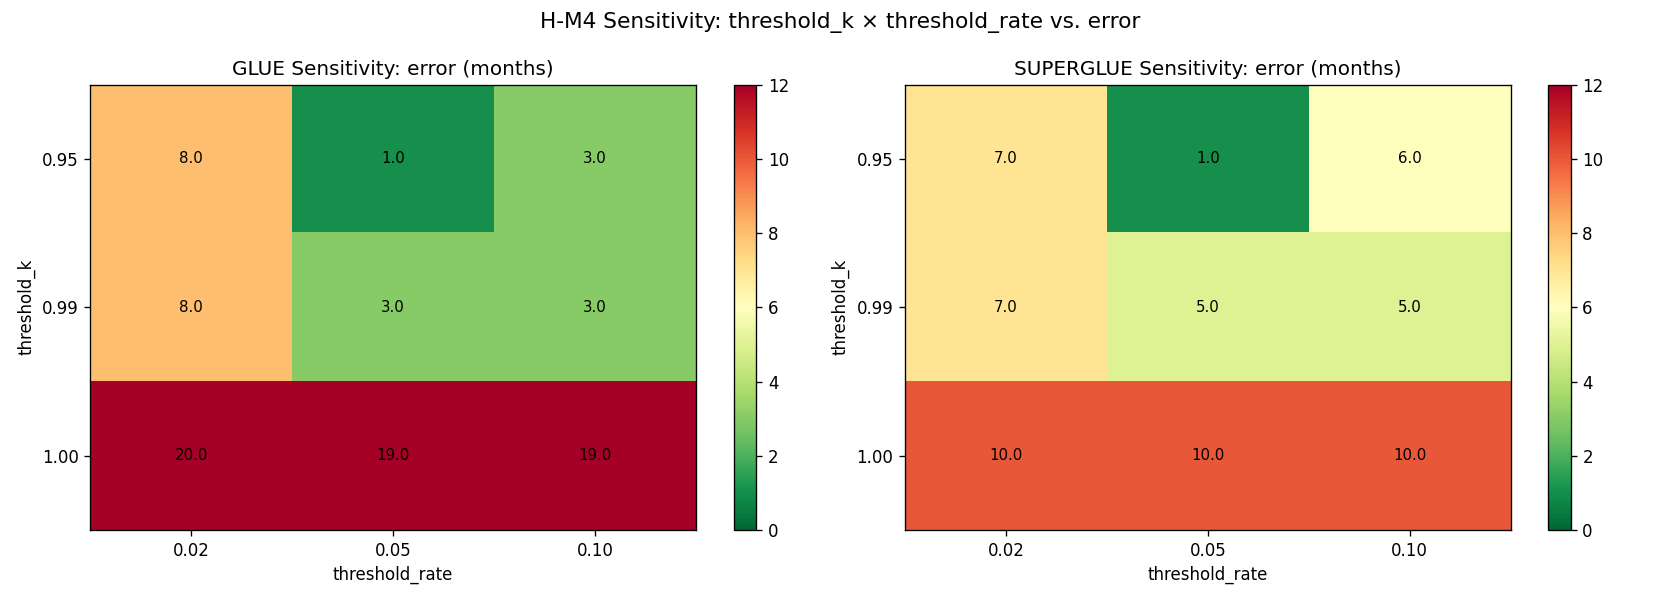
\includegraphics[width=\columnwidth]{figures/h-m4_sensitivity_heatmap.png}
\caption{Sensitivity heatmap for threshold combinations}
\label{fig:h-m4_sensitivity_heatmap}
\end{figure}

\textit{Figure A.1: Heatmap of detection error (months) across the 3 $\times$ 3 threshold grid for GLUE (left) and SuperGLUE (right). The stable low-error region centers on ($\theta _K$ = 0.95--0.99, $\theta _r$ = 0.05).}

\subsubsection{B. Hyperparameter Configuration}

\begin{verbatim}
# Logistic fitting — main pipeline (H-E1, H-M2, H-M3, H-M4)
p0 = [0.92, 0.15, 12.0]
bounds_lower = [0.5, 0.01, -24.0]   # K lower=0.5 (fitting bound); post-hoc plausibility gate checks K >= 0.8
                                      # Compare: H-C1 uses t0_lower=6 (post-launch only for synthetic)
bounds_upper = [1.05, 3.0, 72.0]
maxfev = 10000
bootstrap_n = 500  # fallback when pcov is ill-conditioned

# Saturation detection (H-M4)
threshold_k = 0.99
threshold_k_optimal = 0.95
threshold_rate = 0.05
min_monthly_observations = 12

# Boundary condition experiment (H-C1) — tighter bounds for small synthetic benchmarks
bounds_lower_c1 = [0.8, 0.1, 6]     # t0 >= 6: post-launch only (synthetic data has full S-curve)
                                      # Main pipeline uses t0_lower=-24 to allow pre-launch inflection
bounds_upper_c1 = [1.0, 2.0, 48]
\end{verbatim}

\subsubsection{C. H-C1 Ablation Results}

\textbf{Table C.1: H-C1 ablation variants on small (30--49 entry) synthetic benchmarks.}

\begin{table*}[htbp]
\centering
\resizebox{\dimexpr 2\columnwidth+\columnsep\relax}{!}{%
\begin{tabular}{lllll}
\toprule
Variant & Convergence Rate & Mean $R^2$ & K Boundary Hit Rate & H-C1 Degradation Supported? \\
\midrule
Bounded (primary) & 1.000 & 0.913 & 0.250 & No \\
Strict threshold ($R^2$ < 0.5) & 1.000 & 0.913 & 0.250 & No \\
Loose threshold ($R^2$ < 0.8) & 1.000 & 0.913 & 0.250 & No \\
No bounds & 1.000 & 0.917 & **0.500** & Yes (boundary hit rate exceeds 0.30) \\
Split 30--39 & 1.000 & 0.953 & 0.250 & No \\
Split 40--49 & 1.000 & 0.873 & **0.500** & Yes (boundary hit rate exceeds 0.30) \\
\bottomrule
\end{tabular}
}
\end{table*}

Boundary constraints are the critical factor: removing bounds causes the K-boundary hit rate to exceed 0.30 in both the no-bounds and 40--49 split conditions. The 40--49 sub-group shows greater instability than the 30--39 sub-group, which is counter-intuitive (more data, more instability), suggesting that mid-size benchmarks with more complex noise structure may require particular attention. Real-data validation is needed before these findings can be generalized.

\begin{figure}[htbp]
\centering
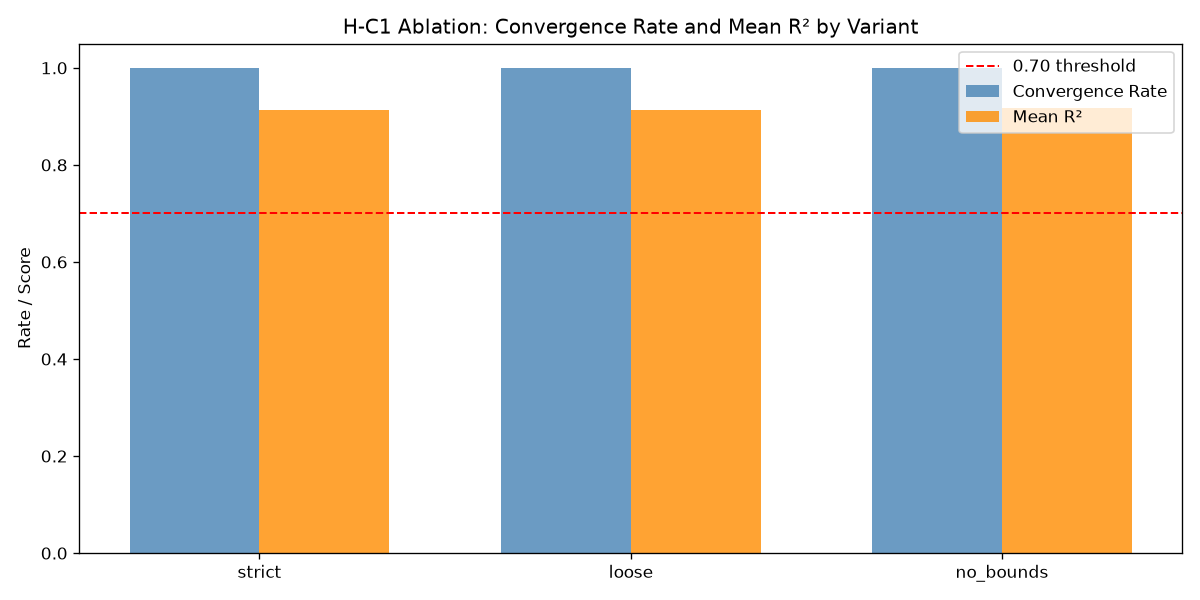
\includegraphics[width=\columnwidth]{figures/h-c1_ablation_summary.png}
\caption{Ablation summary figure}
\label{fig:h-c1_ablation_summary}
\end{figure}

\textit{Figure C.1: Ablation summary showing convergence rate, mean $R^2$, and parameter plausibility across 20 synthetic benchmarks and four variants.}

\begin{figure}[htbp]
\centering
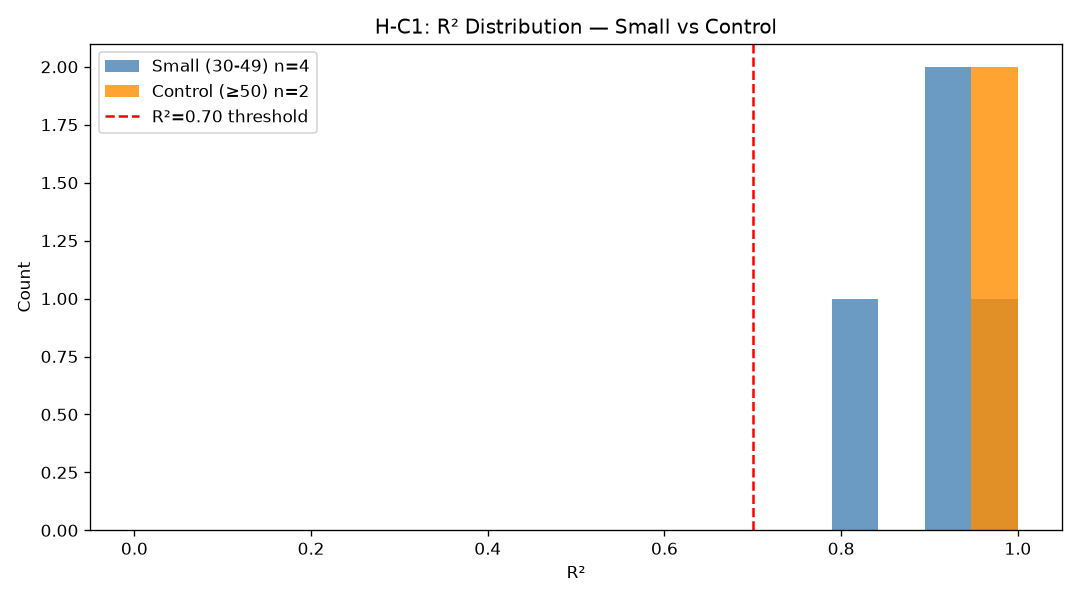
\includegraphics[width=\columnwidth]{figures/h-c1_r2_distribution.png}
\caption{$R^2$ distribution for bounded vs. unbounded fitting}
\label{fig:h-c1_r2_distribution}
\end{figure}

\textit{Figure C.2: $R^2$ distribution across 20 synthetic benchmarks for the bounded (primary) configuration. Mean $R^2$ = 0.913; all benchmarks exceed $R^2$ = 0.70.}
